\begin{titlepage}
    \begin{center}

        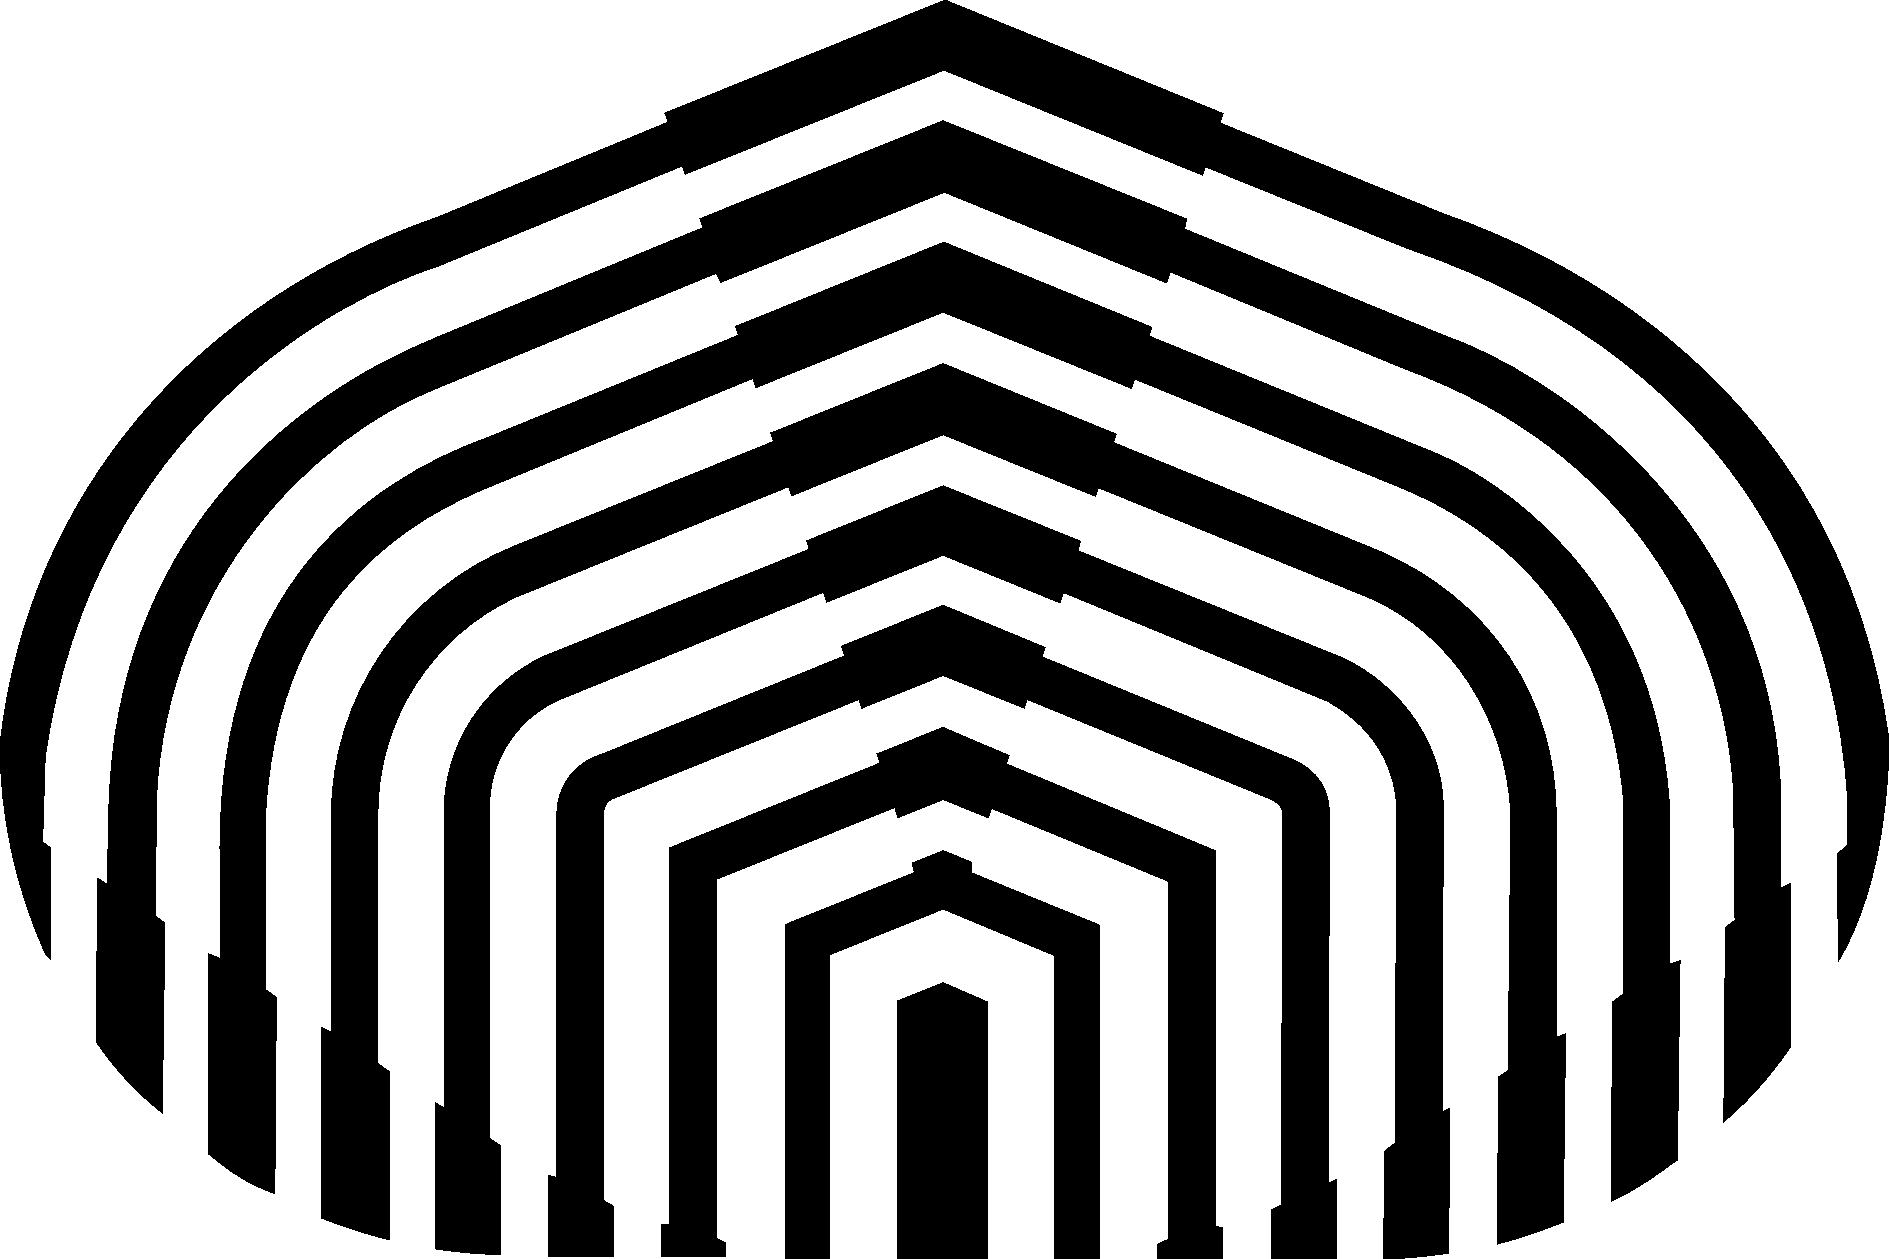
\includegraphics[scale=0.5]{usb.png} \\
        \textsc {\large UNIVERSIDAD SIMÓN BOLÍVAR} \\
        \textsc{DECANATO DE ESTUDIOS PROFESIONALES\\
        COORDINACIÓN DE INGENIERÍA ELECTRÓNICA}\\
        \textbf{IMPLEMENTACIÓN DE SISTEMA DE LOCALIZACIÓN Y MAPEO SIMULTÁNEO (SLAM) A PARTIR DE VISIÓN MONOCULAR Y SENSORES INERCIALES} \\
        PROYECTO DE GRADO \\
        PRESENTADO POR: \\
        Luis Gabriel Lujano Chinchilla, Carnet: 13-10775

    \end{center}
% El resumen debe ser de una sola página
\addtotoc{Resumen}
\abstract
{
	En las tareas de exploración con vehículos autonómos y teleoperados se ha generado la necesidad de desarrollar sistemas capaces de estimar el movimiento del vehículo, la trayectoria recorrida y un mapa de su entorno. Por tanto, se han desarrollado sistemas de odometría y  también de localización y mapeo simultáneo (SLAM, del inglés: \textit{Simultaneous Localization and Mapping}), que cumplan con estos objetivos, basados en diferentes tipos de sensores. En este sentido, el Grupo de Investigación y Desarrollo en Mecatrónica (GIDM) de la Universidad Simón Bolívar ha venido desarrollando un conjunto de proyectos relacionados con los sistemas de navegación de robots autónomos y de operación remota de estos,  en especial de vehículos submarinos. El siguiente trabajo presenta la implementación de un sistema de odometría visual inercial basado en una cámara monocular y una unidad de medición inercial que puede ser utilizado para estimar el movimiento de robots móviles en diferentes ambientes, y que además puede permitir la reconstrucción parcial del entorno del robot. La implementación fue realizada utilizando el Sistema Operativo Robótico (ROS, del inglés: \textit{Robot Operating System}).  Además, se presenta la implementación de un nuevo sistema que permite la generación de secuencias de datos visuales y visuales-inerciales mediante el desarrollo de un robot prototipo terrestre de bajo presupuesto.
	
    \addtocontents{toc}{\vspace{1em}}
   
    
}

% Las palabras clave son generalmente los nombres de áreas de investigación a
% los cuales está asociado el trabajo. Generalmente son tres o cuatro.
\noindent \begin{small} \textbf{Palabras clave}: odometría visual-inercial, SLAM visual-inercial, IMU, cámara monocular, robots, mapa. 
\end{small}
	
% Iniciar nueva página luego del resumen
\clearpage
\setstretch{1.3}

\end{titlepage}
